\chapter{Real-Robot Experiments}

In this chapter, the details of how our experiments are conducted on the real robot are introduced. 
However, due to the complexity of the robot system, the infrastructure built for collecting demonstrations and deploying the neural network policy will be described first. Specifically, a real-time system was built to integrate the camera, grippers, the whole-body controller, and the VR headset. Then, the data collection and neural network policy evaluation results (or lack of thereof) are discussed. 

\section{Infrastructure}

\begin{figure}
	\centering
	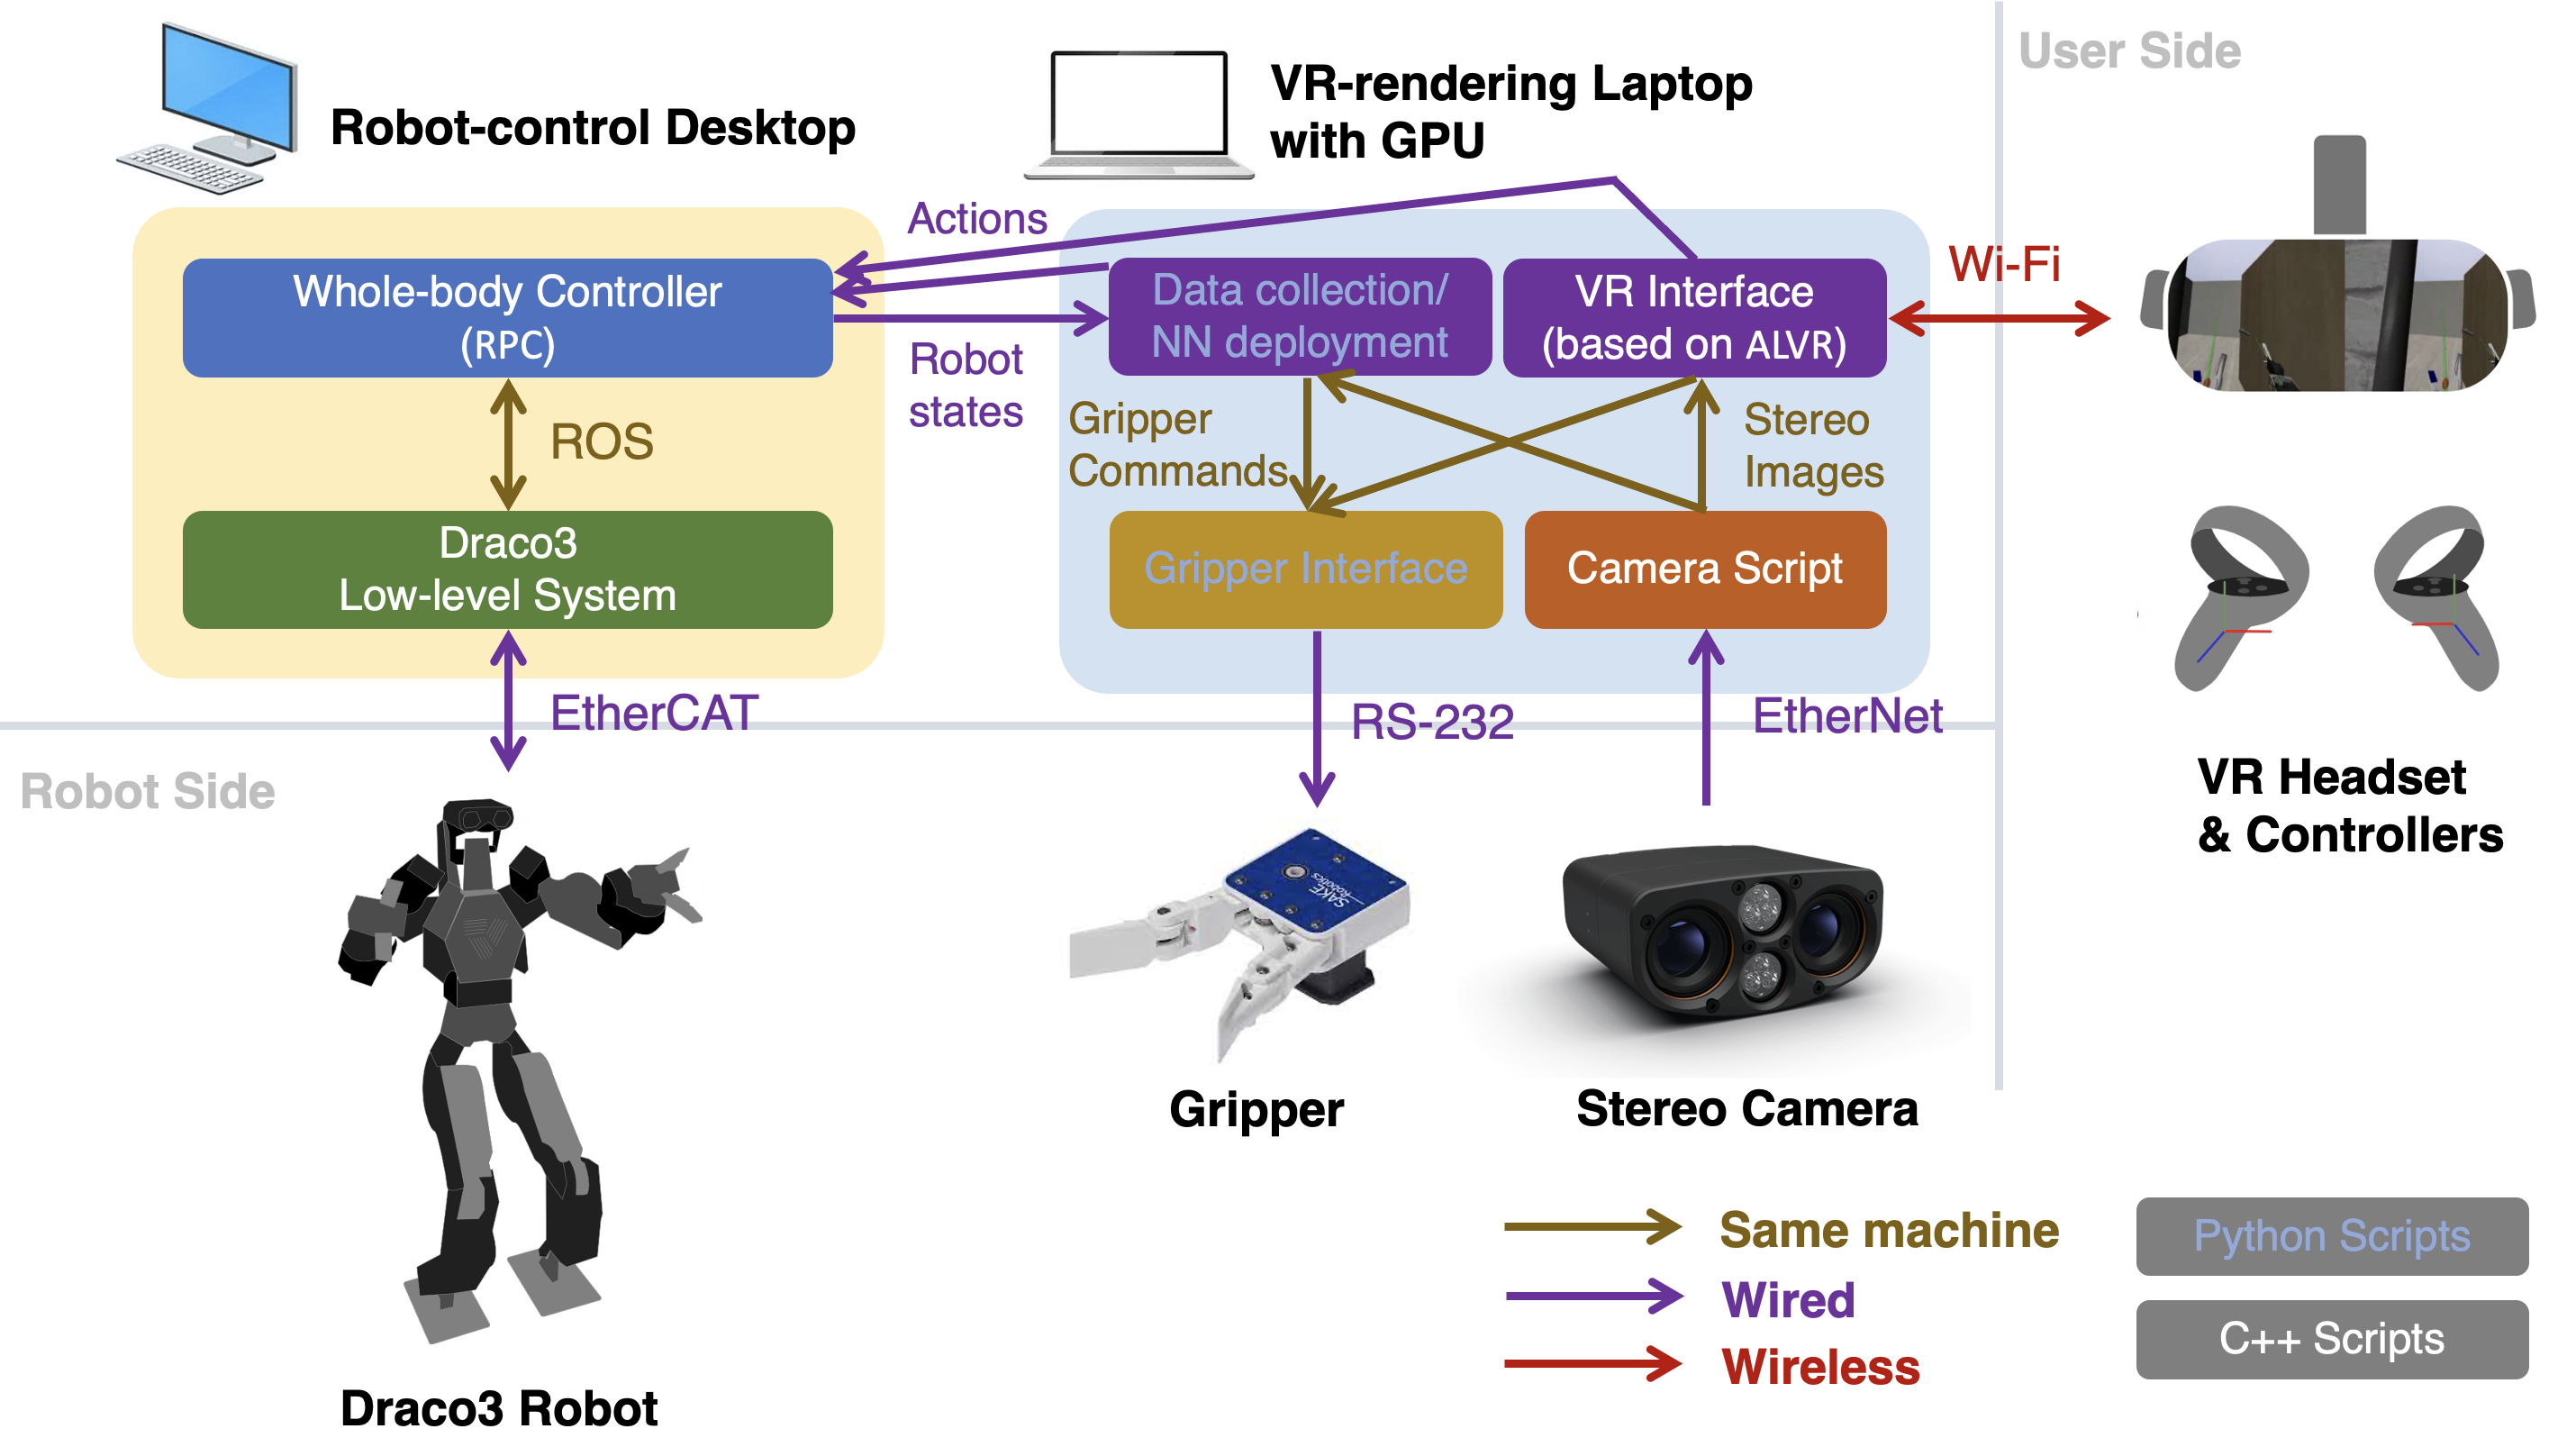
\includegraphics[width=\linewidth]{robot-architecture.png}
    \caption{The infrastructure used to collect demonstraions and deploy policy on the real robot. Original diagram by Mingyo.}
    \label{fig:robot-architecture}
\end{figure}

Figure \ref{fig:robot-architecture} shows the infrastructure for collecting demonstrations and deploying trained policies on the real robot. 
The VR Interface script is the same as before, but more components are added to interface with the grippers, camera, and the robot-control desktop. The whole-body controller running on the desktop is a modified version of PnC \cite{Ahn2021VersatileLP}, named RPC (Robot Planning and Control), created by the hardware team. 

When collecting demonstrations, the camera footage is streamed from the robot's stereo camera to the VR headset. Both RPC and the gripper interface subscribe to VR commands to execute desired actions. The data collection script then pulls robot states from RPC and camera footage from the camera script and saves the resulting data into an HDF5 file. The saved data is then post-processed and used to train the neural network. 
During deployment, the observations (robot states and camera footage) are processed in real-time and fed into the neural network. The processing involves converting hands and feet poses to local frame of the robot and normalizing and resizing images. Then, the neural network inference is performed on the GPU laptop, and the output commands are issued to the grippers and robot. To protect the robot, the output commands are restricted by a 3D bounding box, and the maximum arm movement speed is restricted. 

\subsection{Image Streaming From Camera to VR}

Unlike simulation, the parameters of the camera on the robot cannot be easily adjusted. This means that the interpupillary distance and FOV of the camera does not match those of the human eyes, causing dizziness in the demonstrator \cite{distortion}. Although cropping the images helps with adjusting the convergence distance of the cameras, the difference in interpupillary distance cannot be completely fixed. In addition, there is only RGB data from the left camera, whereas the right camera only has grayscale images. Instead of colorizing the right image from the left image using computer vision techniques, which can produce artifacts that are easily noticeable by the human, we opted to only display grayscale images in the headset. Although the experience isn't very smooth, the depth perception provided by stereoscopic images is still enough to complete many manipulation tasks.

The camera is the MultiSense S7 model from Carnegie Robotics. It comes with a low-level driver library with minimal documentation. RGB image streaming is achieved by executing callback handlers for luma and chroma images on separate threads and merging them together into RGB. Similarly, left and right luma images are streamed in separate threads, which are then synchronized and stitched together to form stereoscopic images. This multi-threaded C++ code is designed to incur minimal image-copying and is thus very efficient.

\section{Neural Network Training and Evaluation}

Our Neural Network takes in the following inputs: stereoscopic images resized to $800\times 200$, positions and velocities of the 26 joints in sin and cos form, the SE(3) poses of the hands and feet in local frame, and the current state machine of the robot, such as balancing or walking forward. A Resnet is trained to extract the image features, and an RNN is used to process the features as well as other inputs to produce an output distribution. The continuous outputs such as hand trajectories are fed into a GMM to produce manipulation commands, while discrete outputs such as locomotion commands and grippers are rounded to either 0 or 1. 

\begin{figure}
	\centering
	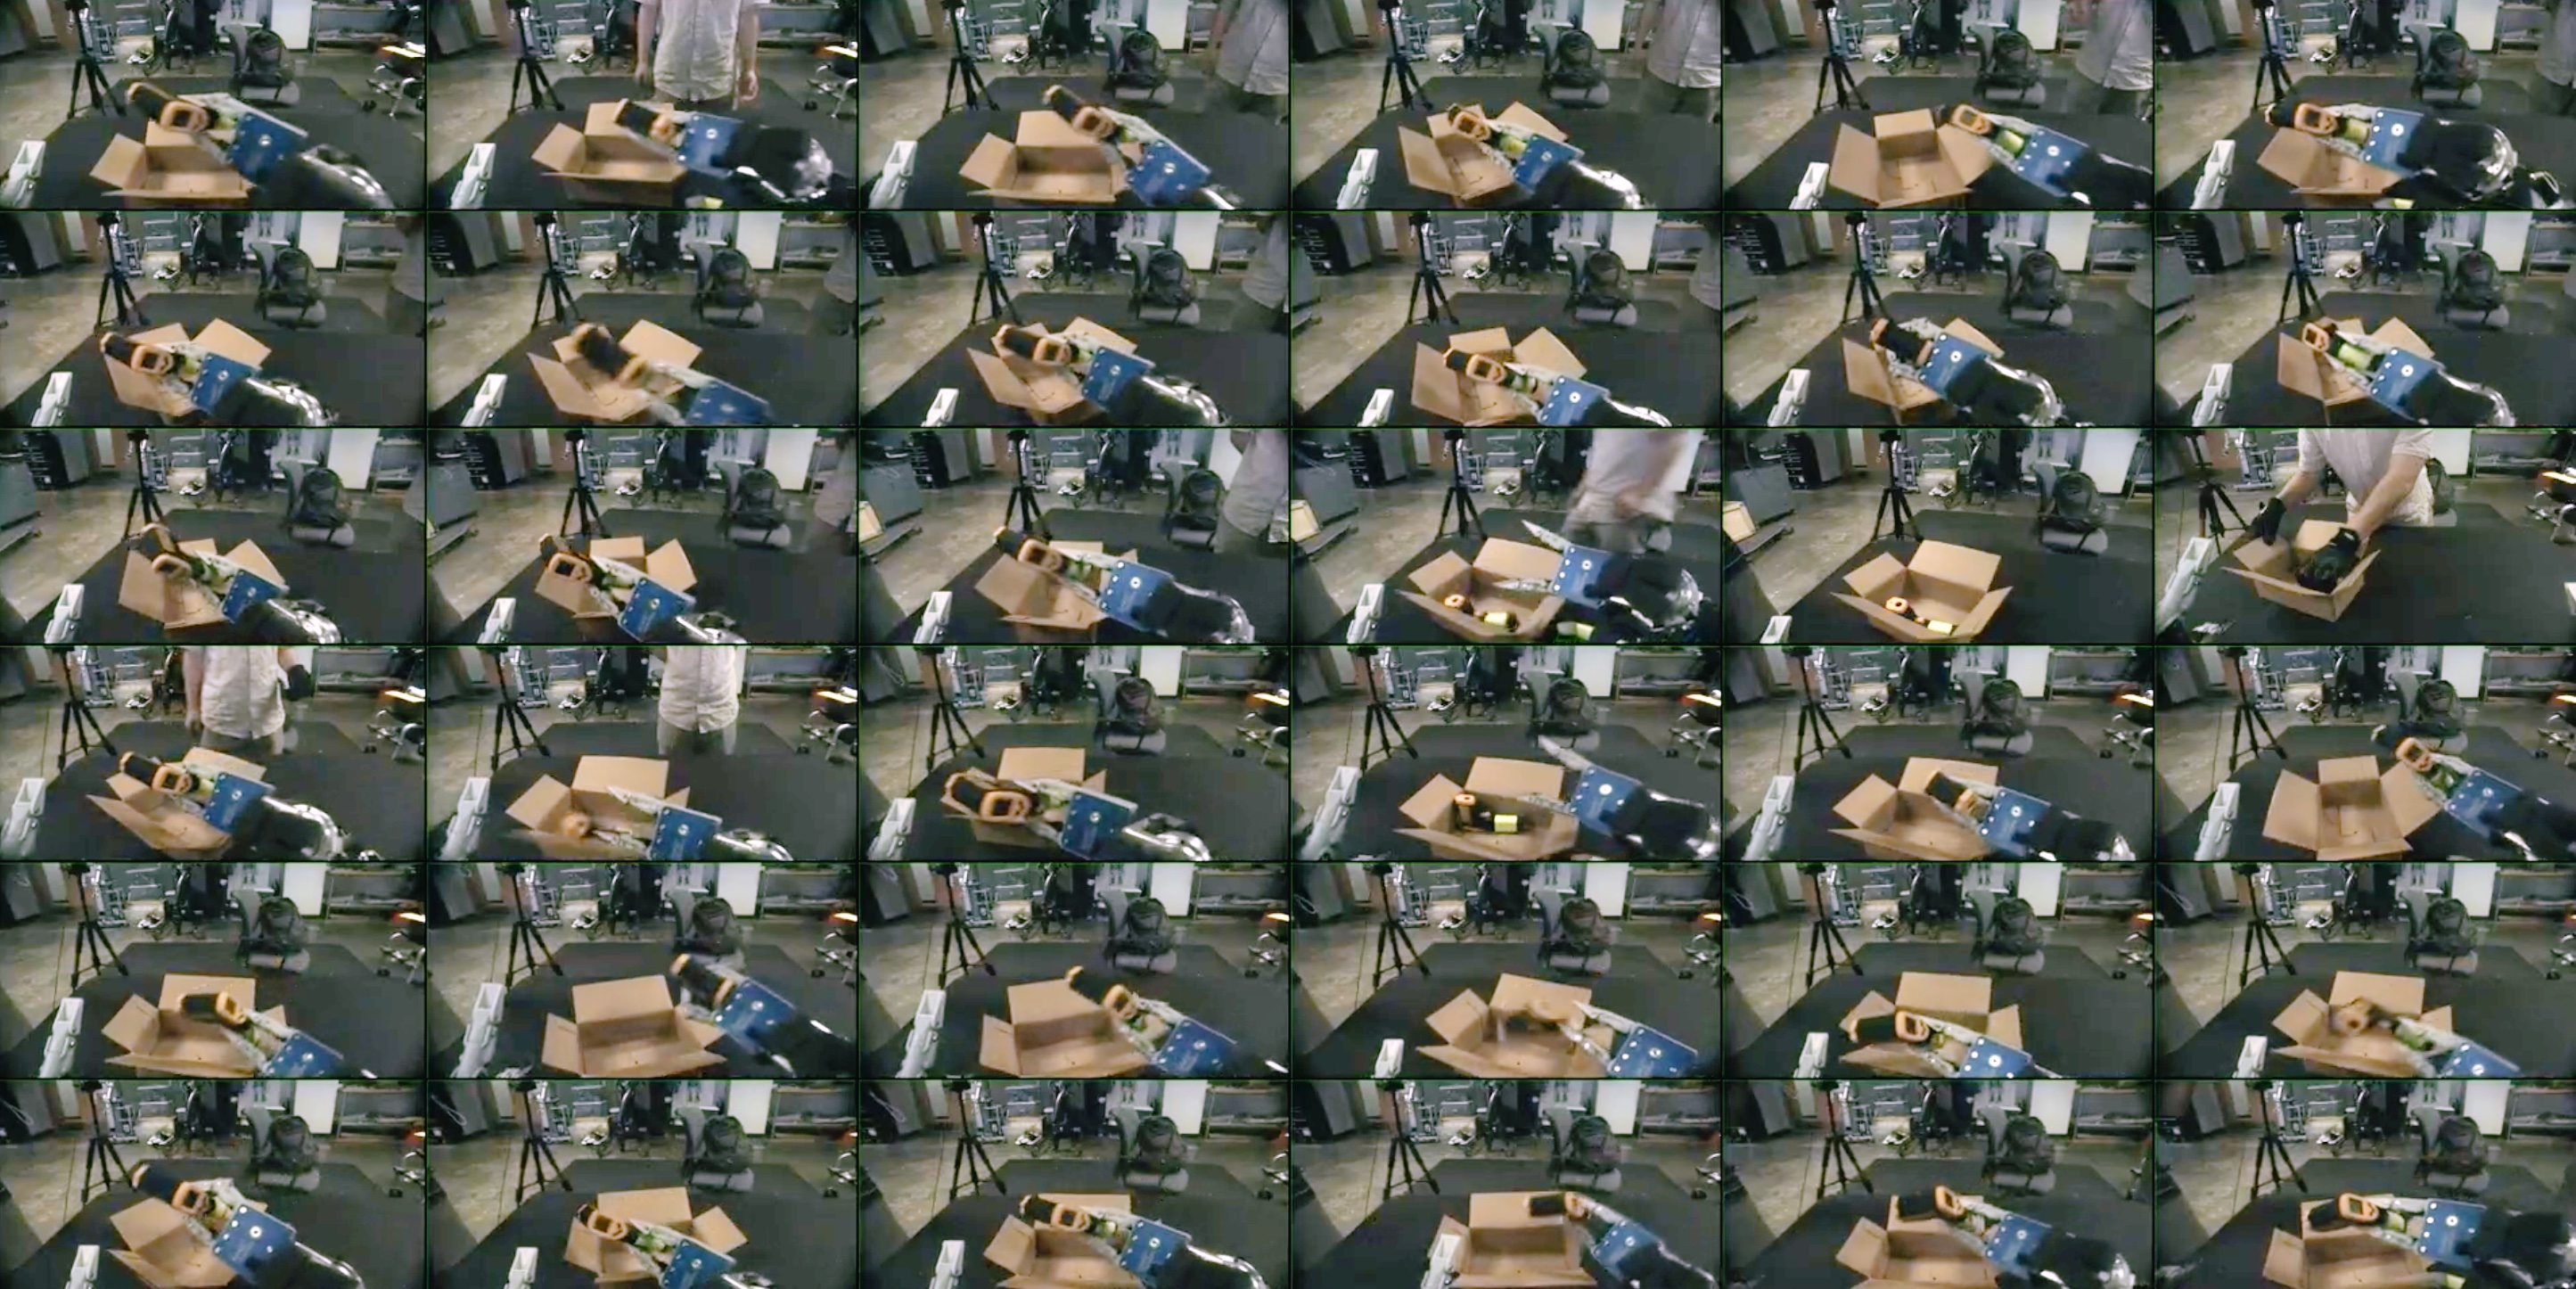
\includegraphics[width=\linewidth]{pick-and-place.jpeg}
    \caption{150 demonstrations of a simple pick-and-place task are collected. The egocentric view for 36 of the episodes are shown. }
    \label{fig:pick-and-place}
\end{figure}

To train the network, 150 demonstrations are collected on a simple pick-and-place task involving grabbing a temperature gun and dropping it in a box, as shown in Figure \ref{fig:pick-and-place}. Since the hardware team is working on replacing the force-torque sensors in the robot's ankles, the robot cannot walk yet. Instead, the task only involves the robot balancing on two feet and doing manipulation with its hands. 

\begin{figure}
	\centering
	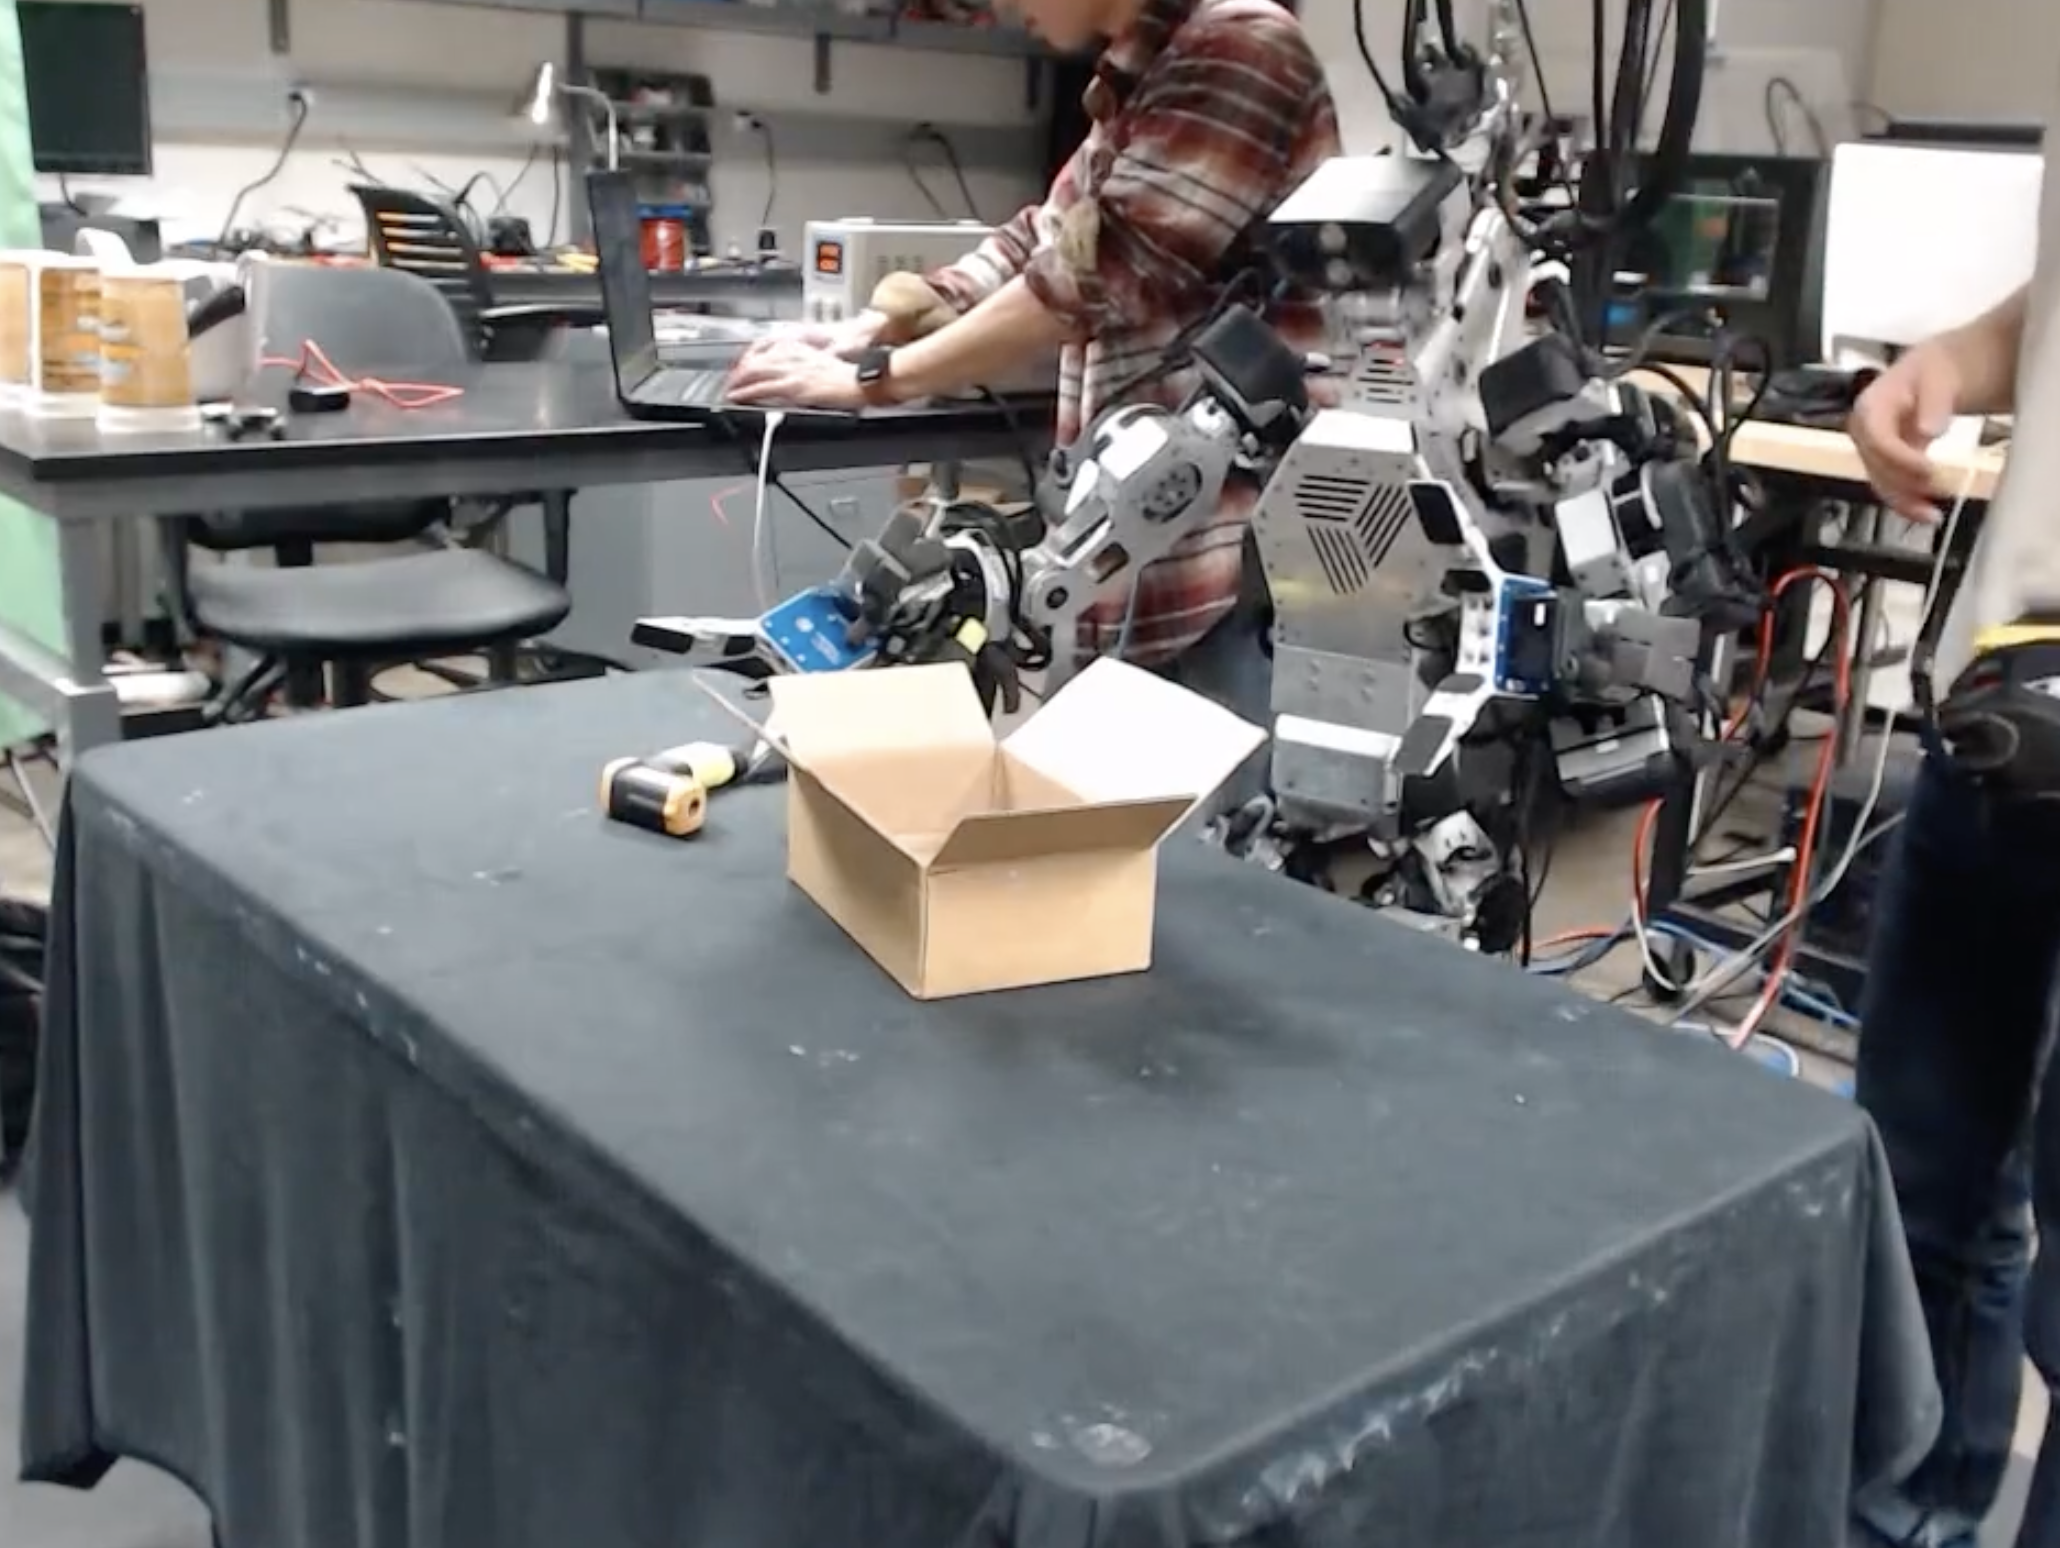
\includegraphics[width=15em]{real-eval.png}
    \caption{During evaluation, the robot usually knocks over the temperature gun before grasping it.}
    \label{fig:real-eval}
\end{figure}
\begin{figure}
	\centering
	\includegraphics[width=\linewidth]{"Right hand orientation.png"}
	\includegraphics[width=\linewidth]{"Right hand position.png"}
    \caption{Plotting the desired (red) vs actual (blue) position and orientation of the right hand during deployment. For each grid, the top row is position and the bottom row is velocity.}
    \label{fig:tracking-plot}
\end{figure}


However, the evaluation of the trained policy is not very successful. Out of 20 evaluations, the robot is only able to pick up the temperature gun in 1 episode. As shown in Figure \ref{fig:real-eval}, the robot fails to locate the object and often knocks it over. 

We hypothesize that the tracking error of the whole-body controller is partially responsible for the difficulty to learn precise manipulation. Figure \ref{fig:tracking-plot} shows whole-body control's tracking error of the right hand during deployment. The red line is the desired pose, and the blue line is the actual pose. Each bump corresponds to a new episode, and the large spikes on the orientation are due to resetting the robot after a failed episode. Since the blue line changes as soon as the red line changes, we know that the tracking is very fast, unlike what we have in simulation. However, the steady-state error is quite large. In the $y$ direction, there can be an up to 10 centimeters error for the hand position. Steady-state error is caused by the lower weight assigned to the hand-tracking task in comparison to the center-of-mass task. In order to maintain balance, the whole-body controller refuses to extend the arm too far forward. This can be fixed by assigning a higher weight to the hand task, but this would trade off the stability of the robot. 

Nonetheless, the policy should learn to compensate for the tracking error, as it has done in simulation. We have also noticed that the policy doesn't vary its actions when the object is placed in different places. We are currently still working on debugging the neural network deployment, but unfortunately, due to the frequent need to repair the robot, we are not able to solve it by the thesis due date. However, the difficulty of performing real-robot experiments on a humanoid platform is the very reason we started out with simulation. Indeed, our method achieves much better results in simulation.
